\chapter{Applicaton to dispersed phase simulations in BIMER}
	\label{ch9:BIMER_lagrangian}

\section{Introduction}

The flowchart of the models from Figure \ref{fig:SLI_graphic_description} applied to BIMER is shown in $\S$\ref{sec:ch9_BIMER_SLI_flowchart}.

\begin{table}[!h]
\centering
\caption{Operating point to perform gaseous and two-phase simulations tested by \citeColor[renaud_high-speed_2015]}
\begin{tabular}{|c|c|c|c|}
\hline
\multicolumn{4}{|c|}{\textbf{Air properties}} \\
\hline
$\dot{m}_g$ [g s$^{-1}$] & $T_g$ [K] & $\rho_g$ [kg m$^{-3}$]  & $\mu_g$ [Pa s]  \\
\hline
43.1 & 433 & 0.816382 & $2.3911 \cdot 10^{-5}$ \\
\hline
\hline
\multicolumn{4}{|c|}{\textbf{Liquid properties}} \\
\hline
$\dot{m}_l$ [g s$^{-1}$] & $\rho_l$ [kg m$^{-3}]$   & $\mu_l$ [Pa s]   & $\sigma$ [N/m]   \\
\hline
1.64 & 750 & $1.36 \cdot 10^{-3}$ & $25.35 \cdot 10^{-3}$ \\
\hline
\hline
\multicolumn{4}{|c|}{\textbf{Burner staging}} \\
\hline
$\alpha$ [$\%$] & $\dot{m}_{l,pilot}$ & $\dot{m}_{l,takeoff}$ & \\
\hline
15 & 0.25 & 1.39 & \\
\hline
\end{tabular}
\label{tab:liquid_operating_point_Renaud}
\end{table}




\section{Computational setup}

For performing dispersed phase simulations, the operating point defined in Table \ref{tab:liquid_operating_point_Renaud} is simulated. The staging factor is $\alpha = 15$, meaning that $15 \%$ of the total liquid flow rate is injected through the pilot stage and the remaining liquid through the multipoint. For total flow rate of $\dot{m}_l = 1.64 g s^{-1}$, the multipoint stage injects a total $\dot{m}_{l,takeoff} = 1.39 g s^{-1}$ (hence $0.139 g s^{-1}$ per injector), and a value of $\dot{m}_{l,pilot} = 0.25 g s^{-1}$ is introduced through the pilot stage.

\subsection{Multipoint stage injection}

For the multipoint stage, the injectors obtained in Chapter \ref{ch:bimer_resolved_atomization} ($\S$ \textbf{Section??}) are used. These injectors were, however, obtained from the simulations of one single injector. In order to initialise the rest of multipoint injection holes (for a total of 10 in BIMER, see Figure \textbf{Figure??}), new numerical injectors need to be defined in each hole by making a revolution of the available ones. This revolution is possible due to the radial of BIMER in terms of injectors location (which are equally spaced to a distance of 25 mm from the center with a radial difference of 36 $\degree$) and the multipoint vane locations: each injection hole is located at the same location between two vanes, hence seeing the same incoming air (see Figure \textbf{Figure??})).

Each injector will deliver a mass flow rate of $\dot{m}_{l,takeoff} = 0.139 g s^{-1}$, equivalent to a flow rate of $Q_l = 185.3 mm^3 s^{-1}$.


\subsection{Pilot stage injection}

Since pilot stage has not been simulated with the injection models developed in this thesis, another methodology must be employed. Given that the pilot of BIMER injects fuel following a hollow cone configuration, the LISA model will be used \citepColor[guedot_developpement_2015]. 

The input parameters for the LISA model to inject a hollow cone spray are summarized in Table \ref{tab:LISA_model_parameters}. They intend to replicate the pilot injection by \citeColor[renaud_high-speed_2015]. For the angle, an initial value of 30 $\degree$ is chosen (Stefano first guess), it can be iterated as we keep on refining the simulations. For the rayon, I have no idea what to do.

For the injection diameter, the following correlation used by Lefebvre for pressure-swirl sprays is used:

\begin{equation}
SMD = 2.25 \left( \sigma \dot{m}_f \mu_l \right)^{0.25} \rho_g^{-0.25}  \Delta P^{-0.5}
\end{equation}

where $\Delta P$ is the pressure drop in the pilot nozzle. According to \citeColor[renaud_high-speed_2015], (p. 24, or 46 PDF), pilot liquid is injected at $2.7 MPa$ to the chamber at atmospheric pressure. By taking this pressure drop, and using the values given in Table \ref{tab:liquid_operating_point_Renaud}, this correlation provides a SMD of $15 \mu m$ (\textbf{CHECK THIS}).

\subsubsection*{LISA model for injection}

For performing pilot injection, the LISA model available in YALES2 is used \citepColor[guedot_developpement_2015]. 

\begin{equation}
X = \frac{A_a}{A_0} = \left( \frac{R_a}{R_0} \right)^2 \frac{\sin^2 \gamma_s}{1 + \cos^2 \gamma_s}
\end{equation}

where $R_a$ is the minimum injection radius, $R_0$ the maximum, and $\gamma_s$ is the mean injection angle. The inputs to the model are $\gamma_s$ and $R_0$, so from the previous equation $X$ can be obtained and the radius $R_a$ can be solved:

\begin{equation}
R_a^2 = R_0^2 X
\end{equation}

The axial velocity imposed to the particles $u_x$ is obtained through the following expression:

\begin{equation}
u_x = \frac{\dot{m}}{\rho_l \pi \left( R_0^2 - R_a^2 \right)} = \frac{\dot{m}}{\rho_l \pi R_0^2 \left( 1 - X^2 \right)} 
\end{equation}

\textbf{OJO}: in Renaud's application case ($\dot{m} = 0.25 ~ g/s$, see Table \ref{tab:LISA_model_parameters}), taking $R_0 = 0.125 ~mm$ gives an axial velocity of $u_x = 7.9 ~ m/s$. This created an almost-point injection, as it can be seen in the simulations. If we take $R_0 = 1.5 ~mm$ (the radius of the hollow cone patch), droplets are injected along all the hollow cone patch. However, the axial velocity imposed is $u_x = 0.05 ~m/s$. So we'll go towards the large radius.

\begin{table}[!h]
\centering
\caption{LISA model setup for pilot injection}
\begin{tabular}{|c|c|}
\hline
\textbf{Parameter} & \textbf{Value} \\
\hline
Mass flow rate $\dot{m} [g s^{-1}]$ & 0.25 \\
\hline
Injector radius $R_0 [mm]$ & 0.125 \\
\hline
Mean angle $\overline{\theta} [\degree]$ & 40 \\
\hline
\end{tabular}
\label{tab:LISA_model_parameters}
\end{table}

\section{Experimental results from literature}

The BIMER operating point tested in this chapter to test the SLI methodology has been chosen since it presents non-reactive experimental results that can be used for validation. These ones, shown in the PhD thesis of \citeColor[renaud_high-speed_2015], consist of the qualitative maps of SMD, axial and vertical velocities shown in Figure \ref{fig:maps_BIMER_renaud_expe_results}. Qualitative experimental results on non-reactive conditions are not available from literature, and hence a qualitative validation is not possible to this date.

\begin{figure}[h!]
\flushleft
\begin{subfigure}[b]{0.3\textwidth}
	\centering
   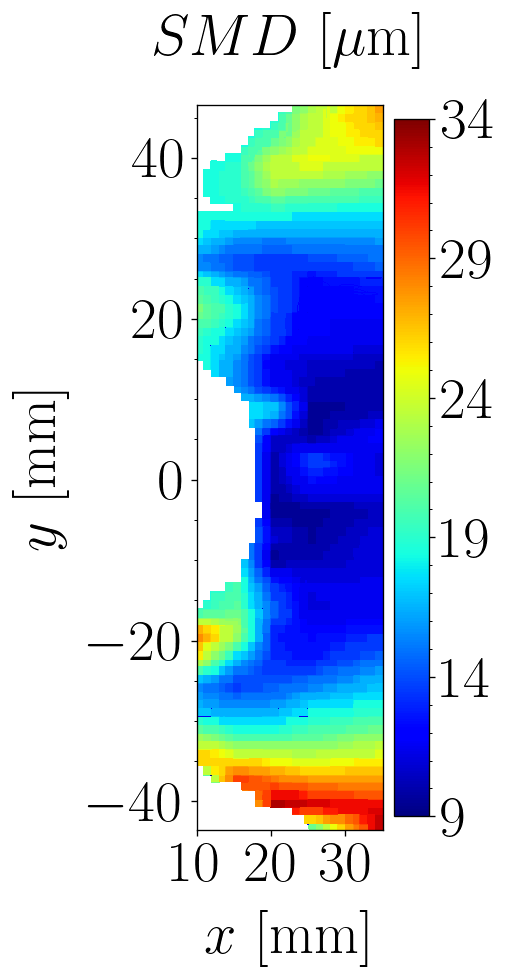
\includegraphics[scale=0.4]{./part3_applications/figures_ch9_lagrangian/expe_maps/SMD_map.png}
   %\caption{Low Weber number operating point.}
   %\label{} 
\end{subfigure}
\hspace*{0.1in}
\begin{subfigure}[b]{0.3\textwidth}
	\centering
   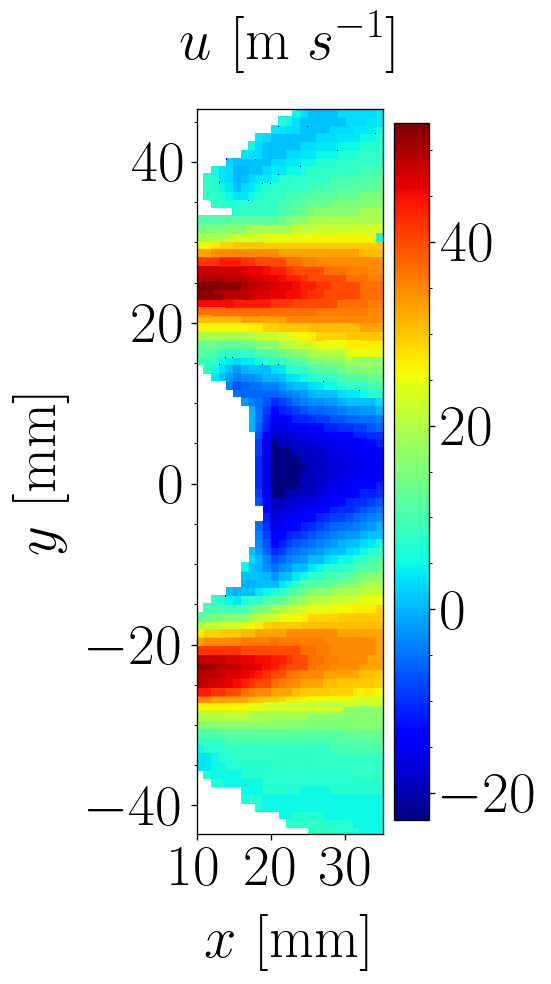
\includegraphics[scale=0.4]{./part3_applications/figures_ch9_lagrangian/expe_maps/u_axial_map.png}
   %\caption{Low Weber number operating point.}
   %\label{} 
\end{subfigure}
\hspace*{0.1in}
\begin{subfigure}[b]{0.3\textwidth}
	\centering
   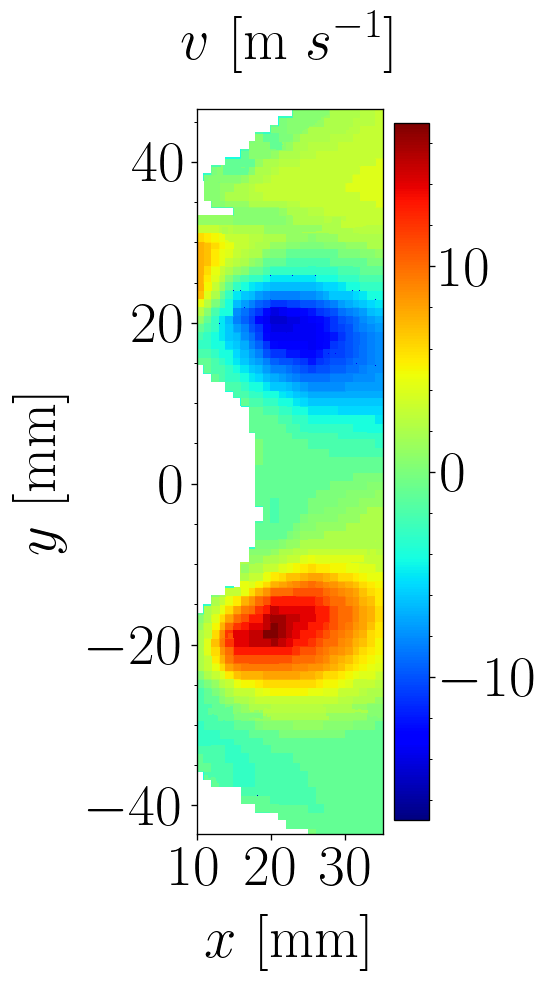
\includegraphics[scale=0.4]{./part3_applications/figures_ch9_lagrangian/expe_maps/u_vertical_map.png}
   %\caption{Low Weber number operating point.}
   %\label{} 
\end{subfigure}
\caption{Experimental maps for for $SMD$, axial velocity $u$ and vertical velocity $v$ from \citeColor[renaud_high-speed_2015].}
\label{fig:maps_BIMER_renaud_expe_results}
\end{figure}

\section{Model flowchart applied to BIMER}
\label{sec:ch9_BIMER_SLI_flowchart}

\section{Injector definition for resolved atomization hole}

\section{Extrapolation of injectors to rest of multipoint holes}

The 

\subsection{Injectors geometry}

\begin{equation}
\boldsymbol{x}_0 =  \begin{pmatrix} - 38.5 ~\mathrm{mm} \\ r \cos \alpha_0 \\ r \sin \alpha_0 \end{pmatrix}
\end{equation}

\begin{equation}
\boldsymbol{x}_i =  \begin{pmatrix} - 38.5 ~\mathrm{mm} \\ r \cos \alpha_i \\ r \sin \alpha_i \end{pmatrix}
\end{equation}


\subsection{General procedure}

\begin{enumerate}

	\item Obtain parameters for SLI of injector 0 (baseline parameters):
	
	\begin{equation}
	\alpha_0  ~~ ; ~~ \boldsymbol{n}_0 ~~ ; ~~ \theta_0 = 90 - \alpha_0 - atan \left( \frac{n_y}{n_z} \right) ~~ ; 
	\end{equation}

	\item Get parameters for SLI of injector $i$ from baseline:
	
	\begin{equation}
	\alpha_i = \alpha_0 - i \Delta \alpha 
	\end{equation}
	
	\begin{equation}
	\boldsymbol{n}_i = 
	\end{equation}
	
	\begin{equation}
	\theta_1 = \theta_0
	\end{equation}
	

\end{enumerate}

\subsection{Definition of coordinate systems and operations}

The global coordinate system is:

\begin{equation}
\boldsymbol{x} =  \begin{pmatrix} x \\ y \\ z \end{pmatrix}
\end{equation}

The local (crossflow) coordinate system is:

\begin{equation}
\boldsymbol{x}^{cr} = \begin{pmatrix} x^c \\ y^c \\ z^c \end{pmatrix}
\end{equation}

with the following equivalences between local and global systems :

\begin{equation}
\boldsymbol{x}^c = \boldsymbol{n}  ~~~~ ; ~~~~ \boldsymbol{z}^c = \boldsymbol{x}  ~~~~ ; ~~~~ \boldsymbol{y}^c =  \boldsymbol{z}^c \times \boldsymbol{x}^c
\end{equation}

where the rotation matrix being:

\begin{equation}
\boldsymbol{R} = \begin{pmatrix} \boldsymbol{x}^{c^T} \\ \boldsymbol{y}^{c^T} \\ \boldsymbol{x}^{c^T} \end{pmatrix}
\end{equation}

More elegantly expresses:

\begin{equation}
\boldsymbol{R} = \begin{pmatrix} x^c_x & x^c_y & x^c_z \\ y^c_x & y^c_y & y^c_z \\ z^c_x & z^c_y & z^c_z \end{pmatrix}
\end{equation}

%\begin{equation}
%\boldsymbol{x} =  \begin{pmatrix} 1 & 2 & -3 \\ 4 & 0 & 1 \end{pmatrix}
%\end{equation}


Transformation for droplet locations is translation + rotation

\begin{equation}
\boldsymbol{x}^c_\mathrm{dr} = \boldsymbol{R} \left( \boldsymbol{x}_\mathrm{dr} -  \boldsymbol{x}_0 \right)
\end{equation}

For droplet velocities, transformation is only rotation:

\begin{equation}
\boldsymbol{u}^c_\mathrm{dr} = \boldsymbol{R} \boldsymbol{u}_\mathrm{dr}
\end{equation}

Inverse transform then:

\begin{equation}
\boldsymbol{x}_\mathrm{inj} = \boldsymbol{x}_0 + \boldsymbol{R}^{-1} \boldsymbol{x}_\mathrm{inj}^c
\end{equation}

\begin{equation}
\boldsymbol{u}_\mathrm{inj} = \boldsymbol{R}^{-1} \boldsymbol{u}_\mathrm{inj}^c
\end{equation}

\section{Conclusion}
